\documentclass{article}

\usepackage{geometry}
\usepackage{amsmath}
\usepackage{graphicx, eso-pic}
\usepackage{listings}
\usepackage{hyperref}
\usepackage{multicol}
\usepackage{fancyhdr}
\pagestyle{fancy}
\fancyhf{}
\hypersetup{ colorlinks=true, linkcolor=black, filecolor=magenta, urlcolor=cyan}
\geometry{ a4paper, total={170mm,257mm}, top=40mm, right=20mm, bottom=20mm, left=20mm}
\setlength{\parindent}{0pt}
\setlength{\parskip}{0.3em}
\renewcommand{\headrulewidth}{0pt}
\AddToShipoutPictureBG{%
  \AtPageUpperLeft{%
    \raisebox{-\height}{
\includegraphics[width=\paperwidth, height=30mm]{../headerarkav.png}}
  }
}
\rfoot{\thepage}
\lfoot{Penyisihan Competitive Programming - Arkavidia 7.0}
\lstset{
    basicstyle=\ttfamily\small,
    columns=fixed,
    extendedchars=true,
    breaklines=true,
    tabsize=2,
    prebreak=\raisebox{0ex}[0ex][0ex]{\ensuremath{\hookleftarrow}},
    frame=none,
    showtabs=false,
    showspaces=false,
    showstringspaces=false,
    prebreak={},
    keywordstyle=\color[rgb]{0.627,0.126,0.941},
    commentstyle=\color[rgb]{0.133,0.545,0.133},
    stringstyle=\color[rgb]{01,0,0},
    captionpos=t,
    escapeinside={(\%}{\%)}
}

\begin{document}

\begin{center}
    \section*{F - Farming Buah} % ganti judul soal

    \begin{tabular}{ | c c | }
        \hline
        Batas Waktu  & 2s \\    % jangan lupa ganti time limit
        Batas Memori & 256MB \\  % jangan lupa ganti memory limit
        \hline
    \end{tabular}
\end{center}

\subsection*{Deskripsi}
Jeremiah memiliki kebun Jeruk yang sebentar lagi akan dipanen buahnya. Saat memanen, Jeremiah harus berjalan kaki mengelilingi kebunnya, yakni \textbf{mengunjungi tempat setiap buah minimal satu kali}. Maka dari itu, dia ingin agar perjalanan yang dilakukan menempuh \textbf{jarak yang minimum}. Bantulah Jeremiah untuk menemukan jarak tempuh minimum yang harus dia lakukan beserta jalurnya. Jika terdapat beberapa jalur yang memiliki jarak minimum, pilihlah yang lebih kecil secara leksikografis.

\begin{center}

\includegraphics[scale=0.4]{baskets.png}

\includegraphics[scale=0.3]{orange.png}
\end{center}

Kebun direpresentasikan dalam bentuk \textit{tree} dengan masing-masing \textit{node} menandakan buah yang harus didatangi untuk dipanen, \textit{edge} dari \textit{tree} menghubungkan 2 buah \textit{node} dan memiliki jarak tertentu.

Jeremiah dapat mulai memetik dari \textit{node} mana saja dan boleh melewati \textit{edge} lebih dari 1 kali.

\textbf{Catatan:}

Sebuah urutan $X_1, X_2, \dots, X_N$ tidak secara leksikografis lebih besar dari $Y_1, Y_2, \dots, Y_M$ jika salah satu dari dua kondisi berikut berlaku:

\begin{itemize}
\item $N \leq M$ dan $X_1 = Y_1, \dots, X_N = Y_N$, yaitu urutan pertama adalah awalan dari urutan kedua

\item Ada posisi $1 \leq j \leq \min(N, M)$, sehingga $X_1 = Y_1, \dots, X_{j-1} = Y_{j-1}$ dan $X_j<Y_j$
\end{itemize}

\subsection*{Format Masukan}
Baris pertama berisi bilangan bulat positif $N$ $(1 \leq N \leq 200000)$, menyatakan banyaknya \textit{node}

$N-1$ baris berikutnya berisi tiga bilangan bulat $U_i, V_i, W_i$ $(1 \leq U_i, V_i \leq N, 1 \leq W_i \leq 10^9)$, menyatakan bahwa \textit{node} $U_i$ terhubung dengan \textit{node} $V_i$ dengan jarak $W_i$

\subsection*{Format Keluaran}
Pada baris pertama, keluarkan sebuah bilangan bulat berupa jarak minimum yang dicari

Pada baris kedua, keluarkan sebuah bilangan bulat $L$, menyatakan banyaknya \textit{node} yang ada pada jalur

Pada baris ketiga, keluarkan $L$ buah \textit{node} yang ada pada jalur yang diminta.

\begin{multicols}{2}
\subsection*{Contoh Masukan}
\begin{lstlisting}
6
1 2 2
2 3 3
3 4 4
2 5 1
2 6 1
\end{lstlisting}
\columnbreak
\subsection*{Contoh Keluaran}
\begin{lstlisting}
13
8
1 2 5 2 6 2 3 4
\end{lstlisting}
\vfill
\null
\end{multicols}


\pagebreak
\subsection*{Penjelasan}

Kebun dapat direpresentasikan sebagai berikut:

\begin{center}
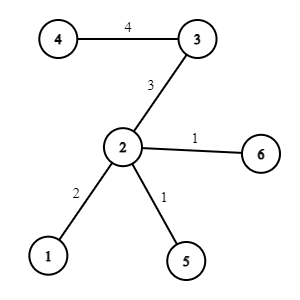
\includegraphics[scale=0.8]{buah.png}
\end{center}

Jarak minimum dengan rute leksikografis terkecil didapat dengan memilih jalur rute:

$$1 \rightarrow 2 \rightarrow 5 \rightarrow 2 \rightarrow 6 \rightarrow 2 \rightarrow 3 \rightarrow 4$$

dengan total jarak: $2+1+1+1+1+3+4=13$

Perhatikan bahwa terdapat jarak minimum dengan memilih jalur rute lain seperti:

$$1 \rightarrow 2 \rightarrow 6 \rightarrow 2 \rightarrow 5 \rightarrow 2 \rightarrow 3 \rightarrow 4$$

namun jalur rute tersebut bukan merupakan jalur rute leksikografis terkecil untuk jarak minimum yang sama, sehingga tidak menjadi jawaban yang benar.

\pagebreak

\end{document}